\documentclass[11pt,a4paper]{article}
\title{Simulation Assignment Report}
\author{Laurens van den Brink 4022831  and Nadia Boudewijn 3700607}
\date{\today}
  \newcommand{\tab}{\hspace*{2em}}
\usepackage{graphicx}
\usepackage{float}

\usepackage{afterpage}
\usepackage[left=5pt,top=5pt,right=5pt]{geometry}
\begin{document}

\begin{titlepage}
\maketitle{}
\end{titlepage}


\tableofcontents
\clearpage



\section{Introduction}
This is report accompanies a simulation model for a production line of DVD's. This simulation model is designed for the Simulation Assignment for the simulation course  2013-2014 at Utrecht University.
\subsection{Problem description}
We will be performing a simulation study for a production line of DVD's, hoping to find improvements for the line. At some points in the line there is limited buffer space and part of the production is batch processing. The producing company wants to find out the best buffer- and batch sizes to increase the dvd production. They are also interested in possible improvements of their production line, especially in alleviating the impact of bottlenecks. 

To gain insight on the production line we questioned the domain expert Marjan van den Akker. She provided us with information about the production process. A schematic overview of the production line can be found on the next page. 


\subsection{Project goal}
The goal is to perform a scientific sound simulation study in order to determine if it's possible to increase the DVD production productivity. 
\section{Problem Analysis}
In this section we will discuss the methods we have used to reach the project goal, as well as some domain-specific issues to this simulation study that need to be adressed. 


\subsection{Assumptions}
A model is supposed to be a simplification of reality, therefore in order to create our model we made some simplifying assumptions that we will discuss in this section. 

\subsubsection{General assumptions}
\begin{itemize}
\item All machines have enough resources available, when they run out, resources are being refilled immediately (which may cause the machine to stop it's production for some time during the refill).
\item The production line runs 24/7, therefore we have chosen a time where after the simulation runs steady. The start-up time from the simulation.
\item When we start the production line we assume none of the machines is broken down.
\item At any moment in time enough repairman are available, so that repairs can be scheduled immediately. 
\end{itemize}

\begin{figure}[H]
\centering
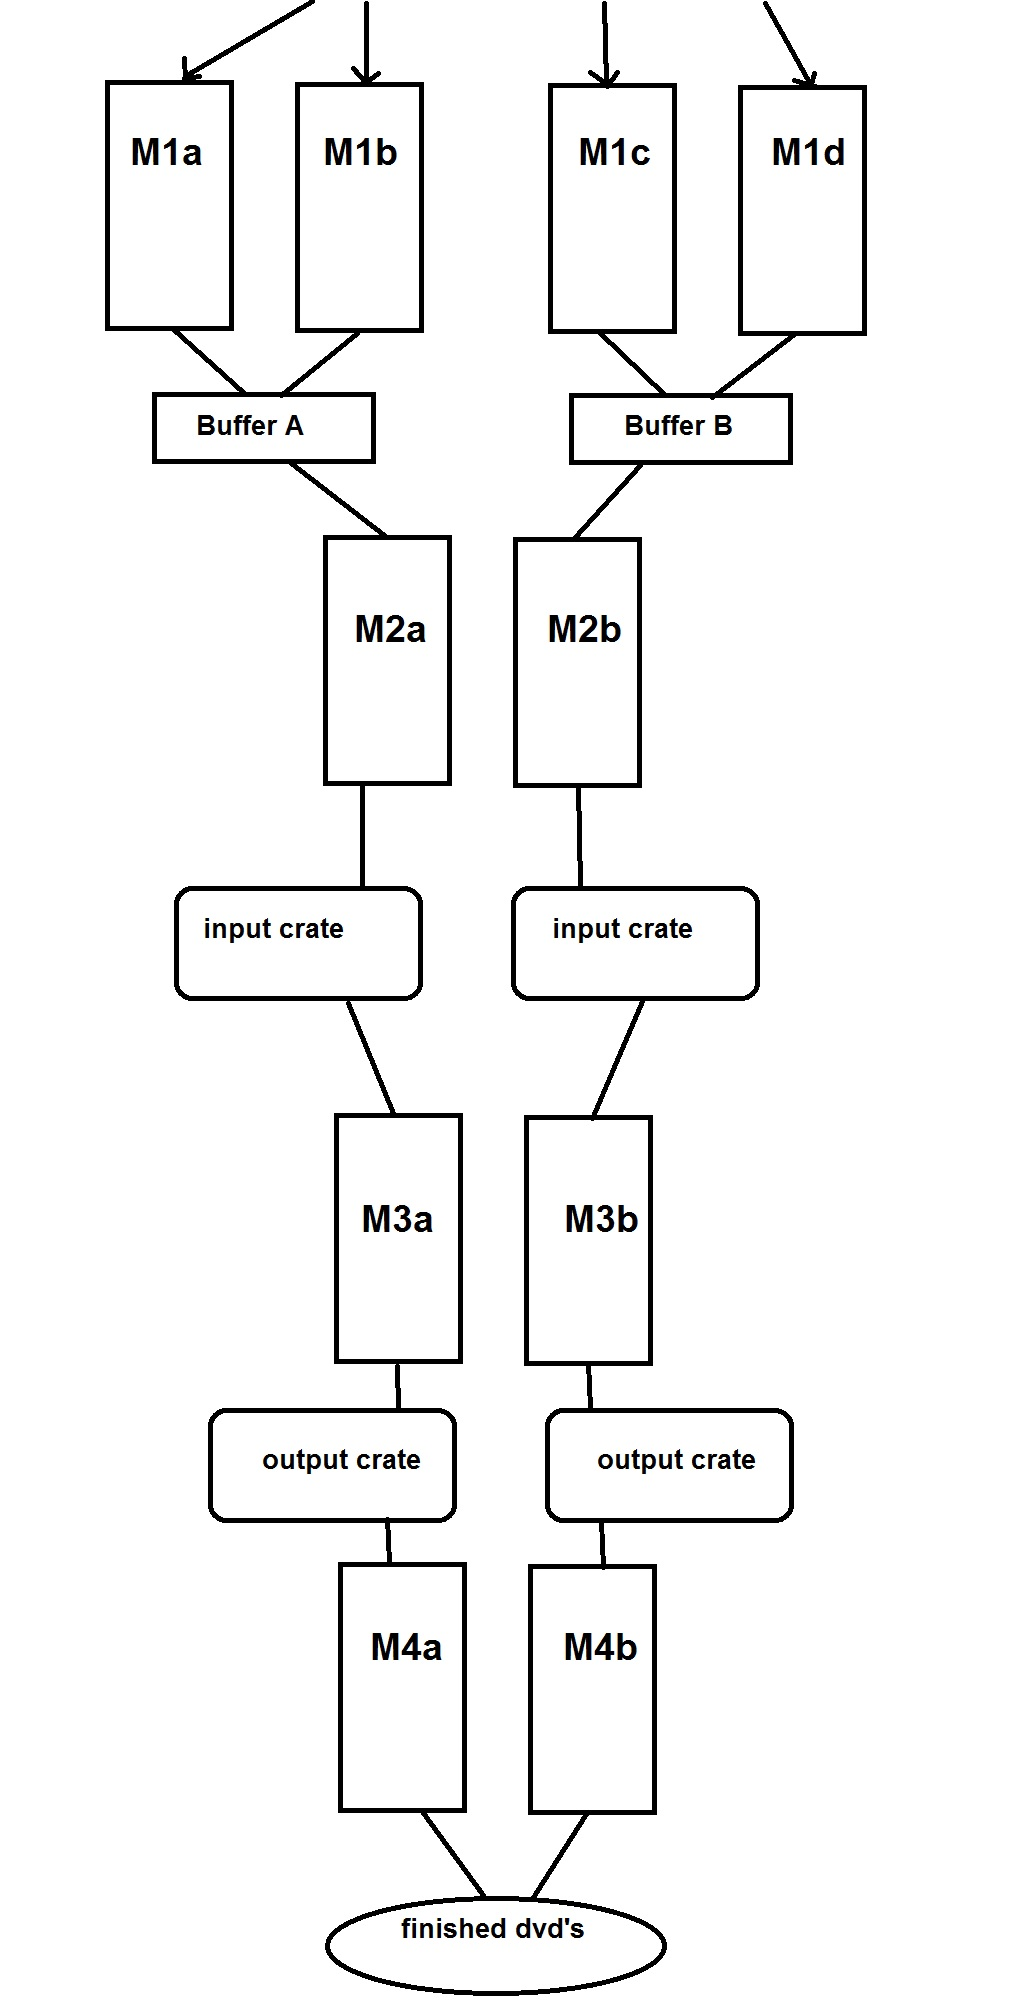
\includegraphics[height = 600 pt]{schemaPL.jpg}
\caption{Figure 1: A schematic representation of the DVD production line.}
\end{figure}

\subsubsection{Disitribution Assumptions}
\begin{itemize}
\item Distributions for time to failure and time to repair are equal for machines of the same sort (machines with the same number in our case).
\item The 500 observations for the processing time of M1/M2/M4 are not enough to run a reliable trace-driven simulation. Therefore we construct an emprical distribution for the processing times of M1/M2/M4 from these observations. 
\end{itemize}


\subsection{Model explanation}
We will start with detailed descriptions of each subsystem in bullet format and how these subsystems interact. Next we will give an overview of the events for this model, and how they are handled. We will also discuss the model state and the performance measures, followed by limitations of the simulation model. 

\subsubsection{M1}
Machine 1 - Injecton Molding
\begin{itemize}
\item There are 4 injection machines (M1a, M1b, M1c, M1d)  that may break down individually. 
\item  A machine will break down every 8 hours on average. We implement this with an exponential distribution on the advice of the expert. 
\item  Repairing a machine takes 2 hours on average. We implement this with an exponential distribution on the advice of the expert. 
\item  There is a buffer (B1) for 20 dvd's between M1a, M1b and M2a. Another buffer (B2) that can hold 20 dvd's is placed between M1c, M1d and M2b. 
\end{itemize}

\subsubsection{Buffer}
\begin{itemize}
\item Buffer A and B can each store 20 DVD's
\item Buffer A can be filled by M1a and M1b, and offers DVD's to M2a
\item Buffer B can be filled by M1c and M1d, and offers DVD's to M2b
\end{itemize}

\subsubsection{M2}
Machine 2 - Dye coating and drying
\begin{itemize}
\item  There are 2 machines, M2a and M2b. 
\item A machine ruins 2% of the dvd's. These dvd's get thrown away at the end of the whole production line. 
\item  There is 5 minutes travel (drying time) between M2 and M3. 
\end{itemize}

\subsubsection{Crate}
\begin{itemize}
\item There are 6 crates.
\item Three of these crates can be filled by M2a and  can go into the production of M3a. The other three crates can be filled by M2b and go into production of M3b.
\item These crates are in te most ideal case: an input, an output and a processing crate. But it is possible for the 3 crates to be all input, or all output but only 1 crate at a time can be processed by a M3 machine. 

\end{itemize}
\subsubsection{M3}
Machine 3 - Sputtering, lacquer coating and drying
\begin{itemize}
\item There are 2 machines, M3a and M3b. 
\item  A machine only works on batches of size 20.
\item A batch is stored in a crate
\item  3 percent of de dvd's are in a delayed batch due to cleaning time of the sputtering part. 
\item  On avergage it takes 5 minutes to clean the sputtering part.  We implement this with an exponential distribution on the advice of the expert. 
\item If the sputtering part doens't have to be cleaned the sputtering takes 10 seconds on average per dvd. We implement this with an exponential distribution on the advice of the expert. 
\item Lacquer coating takes 6 seconds on average per dvd. We implement this with an exponentiall distribution on the advice of the expert. 
\item At the end the whole batch needs 3 minutes of drying before it's ready for output. 
\end{itemize}

\subsubsection{M4}
Machine 4 - Printing and Finishing
\begin{itemize}
\item  There are 2 machines, M4a and M4b. 
\item On average, after printing 200 dvd's the inkt will have to be refilled. We implement this with a normal distribution on the advice of the expert. 
\item Replacing the inkt takes 15 minutes on average, with a standard deviation of 1 minute.
\end{itemize}

\subsubsection{Program Initialization}
\noindent \textbf{MAIN PROGRAM} \textbraceleft\\
	\tab \textbf{while} time $<$ runlenght \\
	\tab \textbraceleft\\
	\tab \tab advance simulation time; \\
	\tab \tab get next event from event list; \\
	\tab \tab update statistics + system state; \\
	\tab \tab generate future events and add them them to event list; \\
	\tab \textbraceright \\
\textbraceright \\


\subsubsection{Events and event handlers}
We distinguish te following events (see event graph on the next page):
\begin{itemize}
\item M1Finished
\item M2Finsihed
\item AddDVDToCrate
\item M3Finished
\item M4Finished
\item BreakdownM1
\item RepairedM1
\item BreakdownM3
\item RepairedM3
\item BreakdownM4
\item RepairedM4
\end{itemize}

\begin{figure}
\center
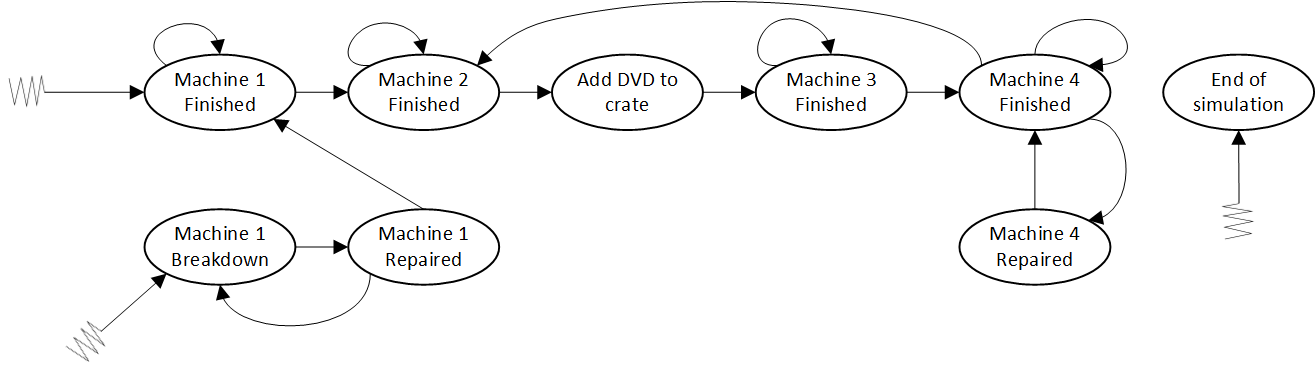
\includegraphics[width = 400 pt]{eventgraph.png}
\caption{ Event graph}
\end{figure}


We use the following \textbf{event handlers} and \emph{subroutines} to deal with the events: \\

\noindent \textbf{Machine 1 Finished:}\textbraceleft\\ 
\tab \textbf{if} (machine state = BROKEN) \textbraceleft \\
		  \tab \tab Store the time the machine should have finished\\
	\tab \textbraceright \\
	\tab \textbf{else if} (machine state = WASBROKEN) \textbraceleft \\
	\tab \tab	the machine has been broken during producing the dvd \\
	\tab \tab	schedule a machine 1 finished event over the time the machine has \tab \tab been repaired\\
	\tab \textbraceright \\
	\tab\textbf{ else if }(machine = machine 1a or machine 1b) \textbraceleft \\
		\tab \tab update bufferA \\
		\tab \tab schedule the next machine 1 finish event to keep producing \\
		\tab \tab\textbf{ if} (machine 2a = IDLE) \textbraceleft \\
                      \tab \tab \tab schedule machine 2a event  \\
		\tab \tab \textbraceright  \\
	\tab \textbraceright \textbf{else} \textbraceleft \\
		\tab \tab update bufferB \\
		\tab \tab schedule the next machine 1 finish event  \\	
		\tab \tab\textbf{ if} (machine 2b = IDLE) \textbraceleft  \\
 		\tab\tab \tab 	schedule machine 2b event  \\
		\tab \tab \textbraceright  \\
	\tab \textbraceright  \\
\textbraceright \\

\noindent \textbf{Schedule Machine 1:} \textbraceleft\\ 
	\tab \emph{the limit of the buffer is 19 when both machines are producing, \\
          \tab otherwise 20} \\
	\tab \textbf{if} (the output buffer is full) \textbraceleft \\
	\tab \tab	state of machine = BLOCKED; \\
	\tab \textbraceright \textbf{else} \textbraceleft \\
	\tab \tab	update dvds in production \\
	\tab \tab 	add machine 1 finished event to event list \\
	\tab \textbraceright \\
\textbraceright \\

\noindent \textbf{Breakdown Machine 1:}\textbraceleft\\  
	\tab MachineState of the machine = BROKEN; \\
	\tab Time machine 1 has broken down = time \\
           \tab schedule repair machine 1: 2 hours exponentially distributed \\
\textbraceright \\

\noindent \textbf{Repair Machine 1: } \textbraceleft\\ 
	\tab schedule breakdown machine 1 \\
	\tab \textbf{if}(the machine did finish in the mean time) \textbraceleft \\
 	\tab \tab delay of machine = Time machine should have finished = time has broken down \\
	\tab \tab machine state of machine = BUSY; \\
	\tab \tab schedule machine 1 finished: over the time the machine has been delayed \\
	\tab \textbraceright \\
	\tab \textbf{else} \textbraceleft \\
	\tab \tab it is not known when the machine should have finished, \\
	\tab \tab so when it happens machine 1 finished event reschedules the event \\
	\tab \textbraceright \\
\textbraceright \\

\noindent \textbf{Schedule Machine 1 breakdown:} \textbraceleft\\ 
	\tab add breakdown machine 1 event to event list in exp(8 hours) \\
\textbraceright \\

\noindent \textbf{Schedule Machine 1 repair:} \textbraceleft  \\
	\tab add repaired machine 1 event to event list in exp(2 hours) \\
\textbraceright \\

\noindent \textbf{Machine 2 Finished:} \textbraceleft\\ 
	\tab schedule AddDVDtoCrate event \\
	\tab schedule next machine 2 finished event
	\tab check if machine was waiting and if so,
	\tab	schedule Machine 1a and 1b or machine 1c and 1d finish event \\
	\tab	(depending on which machine 2 was finished) \\
\textbraceright \\

\noindent \textbf{Schedule Machine 2:} \textbraceleft\\ 
	\tab \emph{check if there is room left within the crates to be filled by m3}\\
	\tab \textbf{if}(dvdReadyforM3 $<=$ crateSize) \textbraceleft \\
	\tab \tab \textbf{if}(buffer $>$ 0) \textbraceleft \\
	\tab \tab \tab update buffer $ -=$ 1 \\
	\tab \tab \tab add machine 2 finished event to the event list \\
	\tab \tab \textbraceright \textbf{else} \textbraceleft \\
	\tab \tab \tab \emph{no input for the machine} \\
	\tab \tab \tab machine state = IDLE; \\
	\tab \tab \textbraceright \\
	\tab \textbraceright \textbf{else} \textbraceleft \\
	\tab \tab \emph{the machine will not be able to output the next dvd} \\
	\tab \tab machine state = BLOCKED; \\
	\tab  \textbraceright \\
\textbraceright \\

\noindent \textbf{ AddDVDtoCrate: }\textbraceleft\\ 
	\tab update dvdReadyforM3 \\
	\tab \textbf{if}(a crate is full and m2 is IDLE) \textbraceleft \\
	\tab \tab schedule machine 3 finished event \\	
	\tab \textbraceright \\
\textbraceright \\

\noindent \textbf{Schedule AddDVDtoCrate:} \textbraceleft\\ 
	\tab add AddToCrate event to event list in 5 minutes \\
\textbraceright \\

\noindent \textbf{Machine 3 Finished:} \textbraceleft\\ 
	\tab update dvd ready for machine 4 with 20 \\
	\tab schedule machine 3 finished event \\
	\tab \textbf{if} machine 4 is IDLE \textbraceleft \\
	\tab \tab schedule machine 4 \\
	\tab \textbraceright \\
\textbraceright \\

\noindent \textbf{Schedule Machine 3:} \textbraceleft\\ 
	\tab \textbf{if}(a full crate is available for input machine 3) \textbraceleft \\
	\tab \tab \emph{start producing this crate} \\
	\tab \tab crates to be filled by machine 3 $=-$ 1 \\
	\tab \tab dvd ready for machine 3 - CrateSize \\
	\tab \tab add machine 3 finished event to event list in exp(10) + exp(6) + 3 $*$ 60 \\
	\tab \textbraceright \textbf{else} \textbraceleft \\
	\tab \tab \emph{output crate and go back to waiting for input} \\
	\tab \tab machine state = IDLE; \\
	\tab \textbraceright \\
\textbraceright \\

\noindent \textbf{Machine 4 Finished:} \textbraceleft\\ 
	\tab update statistics: dvd in production, dvd produced with 98\%, dvd failed with 2\% chance \\
	\tab schedule machine 4 finished event \\
	\tab \textbf{if} (the machine emptied a whole crate) \textbraceleft \\
	\tab \tab crates to be filled by machine 3 $+=$ 1 \\
	\tab \tab \textbf{if}(machine 2 was blocked by no crate available) \textbraceleft \\
	\tab \tab \tab lift the blockade, there is an emtpy crate available again \\
	\tab \tab \textbraceright \\
	\tab \textbraceright \\
\textbraceright \\

\noindent \textbf{Schedule Machine 4:} \textbraceleft\\ 
	\tab \textbf{if}(machine should be serviced) \textbraceleft \\
	\tab \tab machine state = BROKEN; \\
	\tab \tab schedule machine 4 repair event \\
	\tab \textbraceright \textbf{else if}(dvd ready for input machine 4 $>$ 0) \textbraceleft \\
	\tab \tab DvdReadyforInputM4 $=-$ 1 \\
	\tab \tab add machine 4 finished event to event list \\
	\tab \textbraceright \textbf{else if}(crate for other machine 4 is full and the machine isn't working) \textbraceleft \\
	\tab \tab perform a crate switch \\
	\tab \tab DvdReadyforInputM4 $=-$ crate size \\
	\tab \tab add machine 4 finished event to event list\\
	\tab \textbraceright \textbf{else} \textbraceleft \\
	\tab \tab machine state = IDLE \\
	\tab \textbraceright \\
\textbraceright \\

\noindent \textbf{Repair Machine 4:} \textbraceleft\\ 
	\tab reset the dvd counter when service is needed \\
	\tab machine state of machine 4 = BUSY; \\
	\tab schedule machine 4 finished event \\
\textbraceright \\

\noindent \textbf{Schedule Machine 4 Repair:} \textbraceleft\\ 
	\tab add repaired machine 4 event to event list in exp(15 min) \\
\textbraceright \\


	

\subsubsection{Performance measures}
We used the following performance measures:
\begin{itemize}
\item Production per hour: before the simulation study the production was 175 dvd's per hour. We hope to raise this to 200 dvd's per hour. 
\item Throughput time of products 
\end {itemize}


\subsubsection{State}
To keep track of the model state we measure the following:
\begin{itemize}
\item Number of dvd's in production.
\item State of every machine (IDLE / BUSY / BROKEN / WASBROKEN)
\item Buffercontent
\item cratesReadyforInputM3: the amount of crates ready for input M3
\item cratesReadyforInputM4: the number of dvd's that are ready for input M4
\end{itemize}

\subsubsection{Limitations}

\section{Experiments}
Met deze dingen kunnen we rekening houden:
Candidates for sensitivity analysis:
\begin{itemize}
\item the value of a parameter - if it's not sensitive for a specific range of values a better specification is needed
\item  the choice of a distribution
\item  the entity moving thourgh the simulated system - following 1 dvd or a whole batch may produce the same results for the perfomance measures of interest while reducing execution time
\item the level of detail for a subsystem
\item  what data are the most crucial to collect 
\end{itemize}
When one is performing a sensitivity analysis, it is important to use the method of common random numbers to control the randomness in the simulation. Otherwise, the effect of changing one factor may be cofounded with other changes (e.g. different random values from some input distribution) that inadvertently occur.

\subsection{Set up}
Summaries of a data set such as its sample mean and a histogram. Details are for the appendix to retain readability. 
If one has fitted a theoretical probability distribution to a set of observed data, then the adequacy of the representation can be assessed by using the graphical plots and goodness-of-fit tests. 
\subsection{Results}

\subsection{Input Analysis}
Geef een histogram van de frequentieverdeling van de processing tijden.
\afterpage{
\begin{figure}[H]
\centering
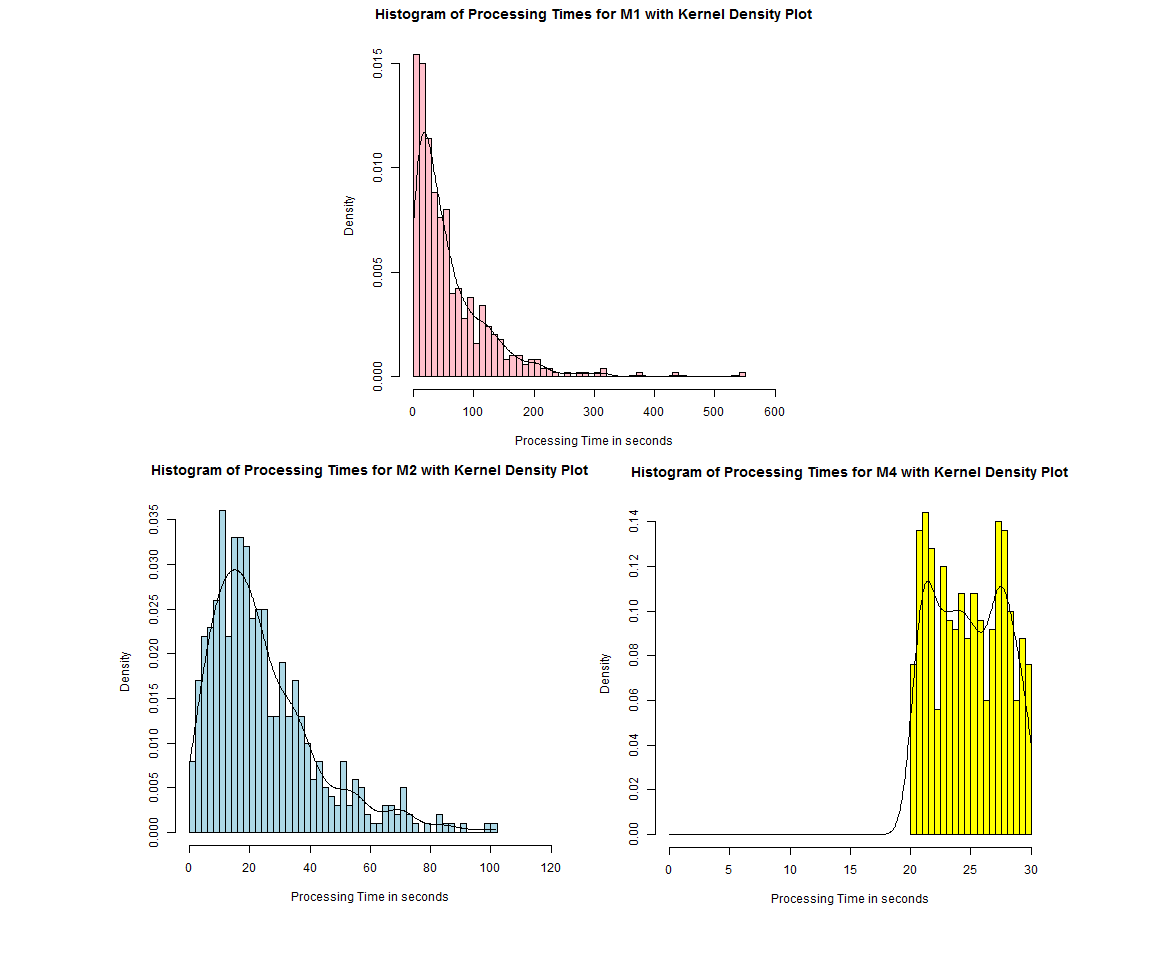
\includegraphics[width = 600 pt]{histograms.png}
\end{figure}
}



\afterpage{
\begin{figure}[H]
\centering
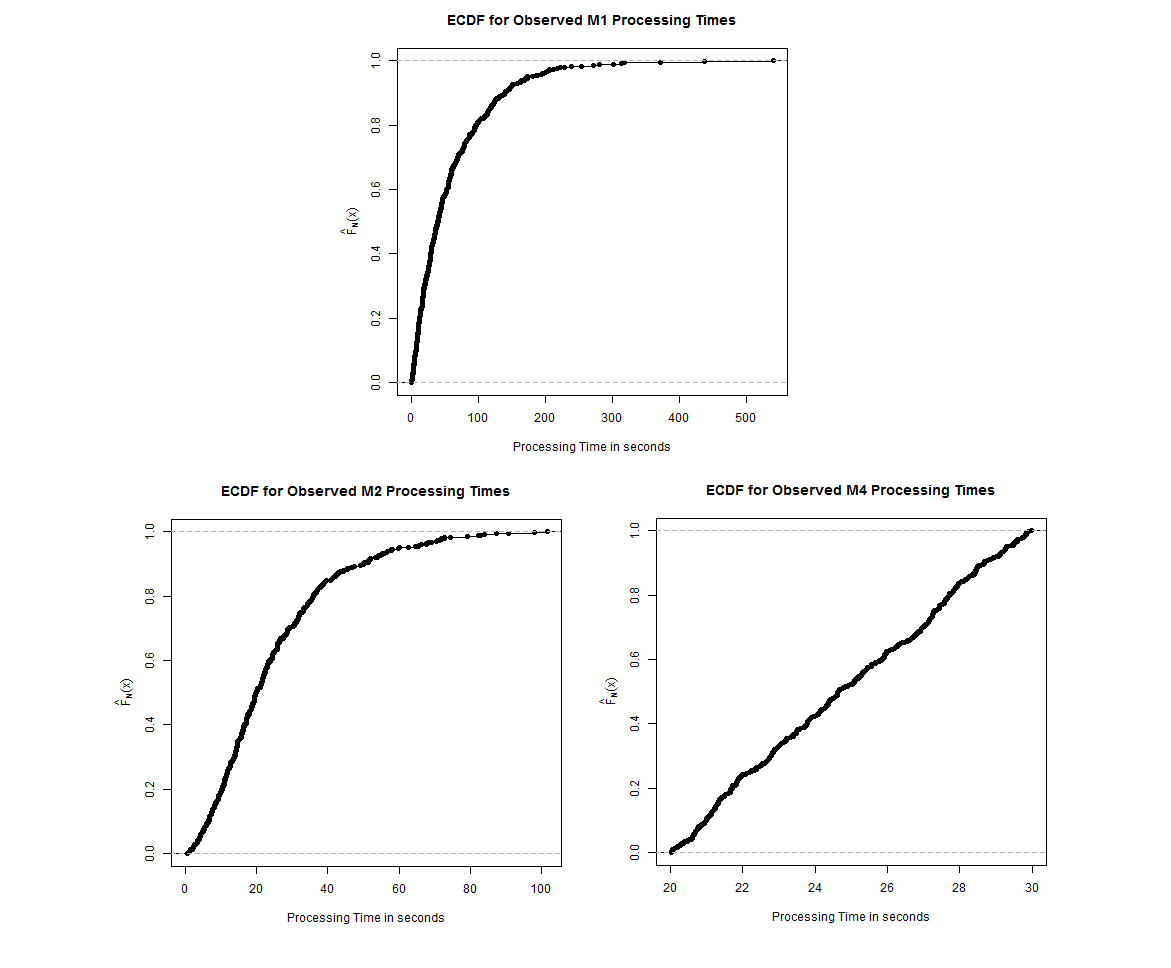
\includegraphics[width = 600 pt]{ecdfs.png}
\end{figure}
}

The goodness of fit of a statistical model describes how well it fits a set of observations.\\
Hypothesis H0: the observations X1,X2,…,Xn follow distribution F\\
Do we accept or reject this hypothesis?

\begin{itemize}
\item Chi-squared test
\item Kolmogorov-Smirnov test
\end{itemize}
Can be performed with R

\subsubsection{ Statistical Hypothesis testing}
\begin{enumerate}
\item Formulate hypothesis Ho
\item Choose type of test
\item Determine significance a and decision rule
\item compute test statistics and take decision
\end{enumerate}

\subsubsection{ Q-Q Plot}

\afterpage{
\begin{figure}[H]
\centering
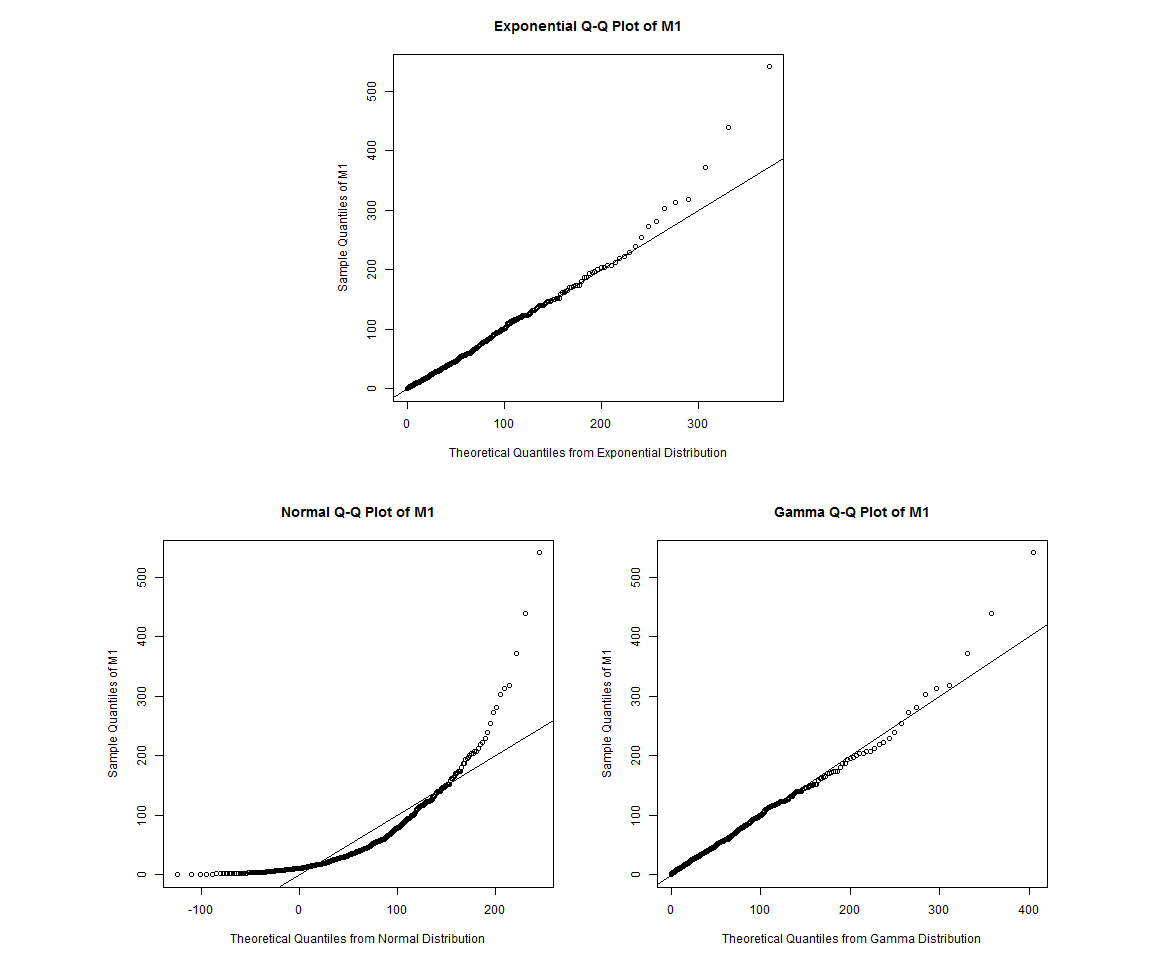
\includegraphics[width=  .8 \textwidth]{qqplots.png}
\end{figure}
}

\subsection{Validation}
Establish that the output data closely resembles the output data that would be expected from the actual system. 


Establish the ability to predict future behavior. Use one data set for calibration and another independent set for validation.



\section{Conclusions}

\section{Appendix}

\subsection{Interview notes}

\subsection{Detailed statistical analyses}





\end{document}

